\section{Persistance locale}

\begin{frame}
\frametitle{La persistance locale}
Objectifs :
\begin{itemize}
\item Persistance des donn\'ees.
\item Pas de d\'eploiement.
\item S\'eparation du mod\`ele et de la persistance.
\item Factorisation du code.
\end{itemize}
\pause
Les solutions :
\begin{itemize}
\item Une base de donn\'ees embarqu\'ee : H2.
\item Un framework : Hibernate.
\item Une architecture en couches.
\item Le pattern DAO.
\end{itemize}
\end{frame}

\begin{frame}
\frametitle{Hibernate}
\begin{center}
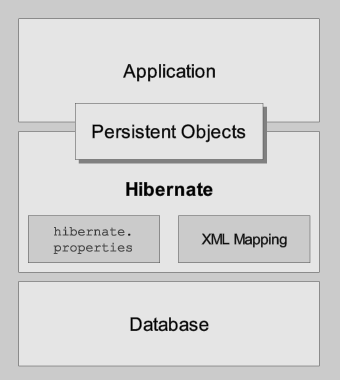
\includegraphics[width=6cm]{images/HibernateArchi}
\end{center}
\end{frame}

\begin{frame}
\begin{itemize}
\item Acc\`es \`a la BD par des appels objets.
\item Configuration sp\'ecifique pour la BD.
\item Deux modes : annotations ou mapping XML.
\end{itemize}
\end{frame}

\begin{frame}[fragile]
Hibernate.cfg.xml
\lstset{breaklines=true, basicstyle=\footnotesize ,  language=XML}
\begin{lstlisting}
<!DOCTYPE hibernate-configuration
    PUBLIC "-//Hibernate/Hibernate Configuration DTD//EN"
    "http://hibernate.sourceforge.net/hibernate-configuration-3.0.dtd">
<hibernate-configuration>
    <session-factory>
        <property name="dialect" >org.hibernate.dialect.H2Dialect</property>
        <property name="show_sql" >true</property>
        <property name="generate_statistics" >true</property>
        <property name="hbm2ddl.auto" >update</property>
        <property name="jdbc.batch_size" >1</property>
     	  <property name="connection.driver_class" >org.h2.Driver</property>
   	  <property name="connection.url" >jdbc:h2:~/Essai</property>
        <property name="connection.username" >sa</property>
        <property name="connection.password" ></property>
   </session-factory>
</hibernate-configuration>
\end{lstlisting}
\end{frame}

\begin{frame}[fragile]
\lstset{breaklines=true, basicstyle=\footnotesize ,  language=XML}
\begin{lstlisting}
<!DOCTYPE hibernate-mapping PUBLIC "-//Hibernate/Hibernate Mapping DTD 3.0//EN" "http://hibernate.sourceforge.net/hibernate-mapping-3.0.dtd">
<hibernate-mapping auto-import="true" package="fr.univnantes.alma.gtd.model.gestionnaireressources">
    <class name="fr.univnantes.alma.gtd.model.gestionnaireressources.Idee" >
        <id name="id" column="ideeId" type="java.lang.Integer">
          <generator class="increment"/>
        </id>
        <property name="nom" type="java.lang.String"/>
        <property name="description" type="java.lang.String"/>
    </class>
</hibernate-mapping>
\end{lstlisting}
\pause
Ajout dans Hibernate.cfg.xml
\begin{lstlisting}
<mapping resource="hibernate/entities/Idee.hbm.xml" />
\end{lstlisting}
\end{frame}

\begin{frame}
\frametitle{Le pattern DAO}
Pattern bas\'e sur Pattern Factory.\\
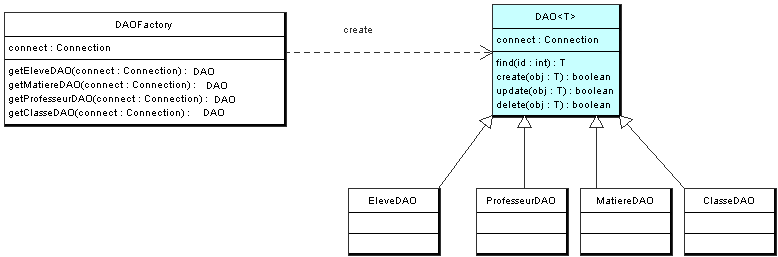
\includegraphics[width=10cm]{images/PatternDAOIdeal}
\end{frame}

\begin{frame}
\frametitle{Le pattern DAO}
TopCased : probl\`eme de templates!
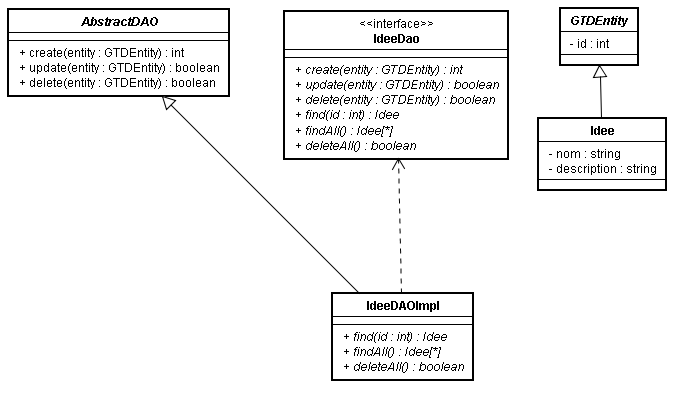
\includegraphics[width=10cm]{images/PatternDAOReel}
\end{frame}

\begin{frame}
\frametitle{La base de donn\'ees}
Creation \'a la vol\'ee par Hibernate.\\
Probl\`emes et solutions :
\begin{itemize} 
\item Une table par hi\'erarchie d'h\'eritage (ex : Pattern Etat).
\item Les relations one-to-one.
\end{itemize}
\end{frame}